%!TEX root = ../main.tex

%
% Notes: 
%
%  exact implementation
%  comparison with rollback at batch N
%  relaxing the solvers
%  dealing with false positives
%
%  running on TPC-C/sanjay's.  equality is easier
%
% Need names for
%  * rollback
%  * exact solution
%  * fixing an individual/batch of queries
%
\section{Experiments}

In this paper, we have described several heuristic algorithms based on decision trees 
and bounding box algorithms, as well as an exact, albeit less-scalable,
constraint-based solution to the \prob problem.  In addition, we 
introduced  several extensions to the CPLEX-based solution that 
1) improve the scalability of the system and 2) tolerate false positives and 
negatives in the input complaint set.
Our goals in the evaluation is to understand these trade-offs in
controlled synthetic scenarios, as well as study the effectiveness
in typical database query workloads based on widely used benchmarks.

To this end, our experiments are organized as follows: First, 
establish the quality limitations of existing heuristics and the need for a formal, 
constraint-based algorithm (\exact).  Second, we study how each of the 
optimizations described in Section~\ref{s:optimiztaions} improves algorithm scalability.
Third, we introduce different forms of error in the input complaint sets and study the 
effectiveness of our noise-handling heuristics.  Finally, we use two
representative database transaction benchmarks, TPC-C XXX~\cite{tpcc} and AuctionMark~\cite{auctionmark}
to study \sys in realistic scenarios.




%
% NOTE: figures are named <experimentsection>_<subsection>_<xaxis>.pdf
%

\subsection{Experimental Setup}


\begin{table}[t]\small
  \centering
  \begin{tabular}{c|l|c}
  {\bf Param} & {\bf Description} & {\bf Default} \\
  $V_d$  & Domain range of the attributes  & $[0, 100]$ \\
  $N_D$  & \# tuples in final database & $1000$ \\
  $N_a$  & \# attributes in database & $10$ \\
  $N_w$  & \# predicates in \texttt{WHERE} clauses & $1$ \\
  $N_s$  & \# \texttt{SET} clauses & $1$ \\
  $N_q$  & \# queries in query log & $100$ \\
  $idx$  & Index (backwards from most recent) & $\{0, 25, 50,$ \\
         & of corrupted query & $100, 200, 250 \}$ \\ %$\frac{N_q}{2}$ \\
  $r$    & Range size of \texttt{UPDATE} queries & 10 \\
  $s$    & Zipf $\alpha$ param of query attributes, & $1$ \\ 
  $set$  & Constant vs relative \texttt{SET} clauses. & const \\ \end{tabular}
         %& power low distribution $P(v) = v^{-s}$ & \\\end{tabular}
  \label{t:params}
  \caption{Experimental Parameters}
\end{table}


\begin{table}[t]\small
  \centering
  \begin{tabular}{c|l}
  {\bf Param} & {\bf Description} \\
  $TP$ & True positive rate: \% of true complaints corrected \\
  $FP$ & False positive rate: \% of errors introduced\\
  $t_{prep}$ & Time to construct CPLEX problem \\
  $t_{send}$ & Time to send CPLEX problem to solver \\
  $t_{solve}$ & Time for solver to generate a solutions\\
  $t_{total}$ & End-to-end execution time \\ 
  $d_{measure}$ & \red{Some sort of distance measure} \\\end{tabular}
  \label{t:metrics}
  \caption{Metrics Compared}
\end{table}



Each of our experiments follows a standard procedure.  
We generate a sequence of queries using a synthetic query generator or 
the benchmark program, and corrupt the query log as described below. 
We then execute the original and corrupt query logs on an initial (possibly empty) database,
and perform a tuple-wise comparison between the resulting database states 
to generate a true complaint set.  
We then add noise to the complaint set by 1) picking random tuples not in the true
complaint set to add false positive complaints, and 2) removing true complaints to simulate false negatives.
Finally, we execute the evaluated algorithms on the complaints and compare the fixed
query log with the true query log, as well as the fixed and true
final database states to measure performance and accuracy metrics.

Tables~\ref{t:params} and~\ref{t:metrics} summarize the key parameters that
we vary throughout our experiments, as well as the metrics we use to evaluate
the quality of the algorithm solutions, respectively.  The rest of this section
outlines our datasets, workloads, and parameters used to generate the synthetic query log.


\subsubsection{Datasets and Workloads}

This subsection describes the query and data generation process in greater detail.

% Anant's workload?

\stitle{TPC-C} We use the data and query workload over the {\it
CUSTOMER} table in TPC-C~\cite{}.  We generate a database at scale
1 with one warehouse, and keep only the queries that modify the
{\it CUSTOMER} table.  We then randomly perturb a subset of the
queries to generate the corrupted query log.
\xlw{Describe how corrupted}

\stitle{AuctionMark} \xlw{Describe benchmark and how queries are corrupted}



\stitle{Synthetic} 
We generate an initial database of $N_D$ random tuples.  
The schema contains $N_a=5$ attributes $a_1\ldots a_5$, whose values are
picked from $V_d$ uniformly at random, along with a primary key $id$.
We then generate a sequence of $N_q$ queries containing a mixture of \texttt{INSERT} queries,
point \texttt{UPDATE} queries, and range \texttt{UPDATE} queries.  
The \texttt{UPDATE} queries have the following respective forms, where \verb|?| is a query parameter 
and \verb|r| is the size of the range.

{\scriptsize
\begin{verbatim}
  UPDATE SET (a_i = ?),.. WHERE a_j = ? AND ...
  UPDATE SET (a_i = ?),.. WHERE a_j in [?, ?+r] AND ...
\end{verbatim}
}

The $set$ parameter controls whether the \texttt{UPDATED} queries set attributes to random constant values ({\it const}),  
or increment attributes by a random amount ({\it rel}).  The \texttt{WHERE} clauses form a conjunction.
In addition we varied a skew parameter $s$, which determines the attributes referenced in the \texttt{WHERE}
and \texttt{SET} clauses.  Each attribute in  a query is picked from a zipfian~\cite{zipf} distribution
with exponent $1+s$.  This allows our experiments to vary between a near-uniform distribution, where each attribute is
equally likely to be picked, and a skewed distribution where nearly all attributes are the same.
\texttt{INSERT} queries simply insert values picked uniformly at random from $V_d$.  

\xlw{Replace with what we actually do:
We first consider three different homogenous query logs: \texttt{INSERT} only ($p_I = 1$), 
\texttt{PK} update only ($p_I = 0, p_{pk} = 1$), and \texttt{RANGE} update only ($p_I = 0, p_{pk} = 0$).
These query logs help us understand \sys's performance characteristics for each query type individually.  
Finally, we investigate heterogenous mixtures of the three query types to simulate varying amounts of real settings.
}

\noindent {\it Effect of Index of Corrupted Query:}
A key parameter for our experiments is the location of the corrupted query ($idx$).  
This parameter deteremines the number of queries \sys must consider when searching for a fix,
and affects the size of the complaint set.  Both of these characteristics directly impact \sys's 
runtime performance. For this reason, it is undesirable to randomly pick and corrupt queries
throughout the query log, as the performance and accuracy results may not be comparable. 
To better understand the relationship between $idx$ and the size of the complaint set, we ran
simulations using a database with $20$ attributes, and a query log of size $1000$ containing
either all $set = const$ or $set = rel$ \texttt{UPDATE} queries.
We varied  $idx$ uniformly throughout the query log, and additionally varied
the skew $s$ and range $r$ parameters to study how they affect the size of the complaint sets.


  \begin{figure}[h]
  \centering
  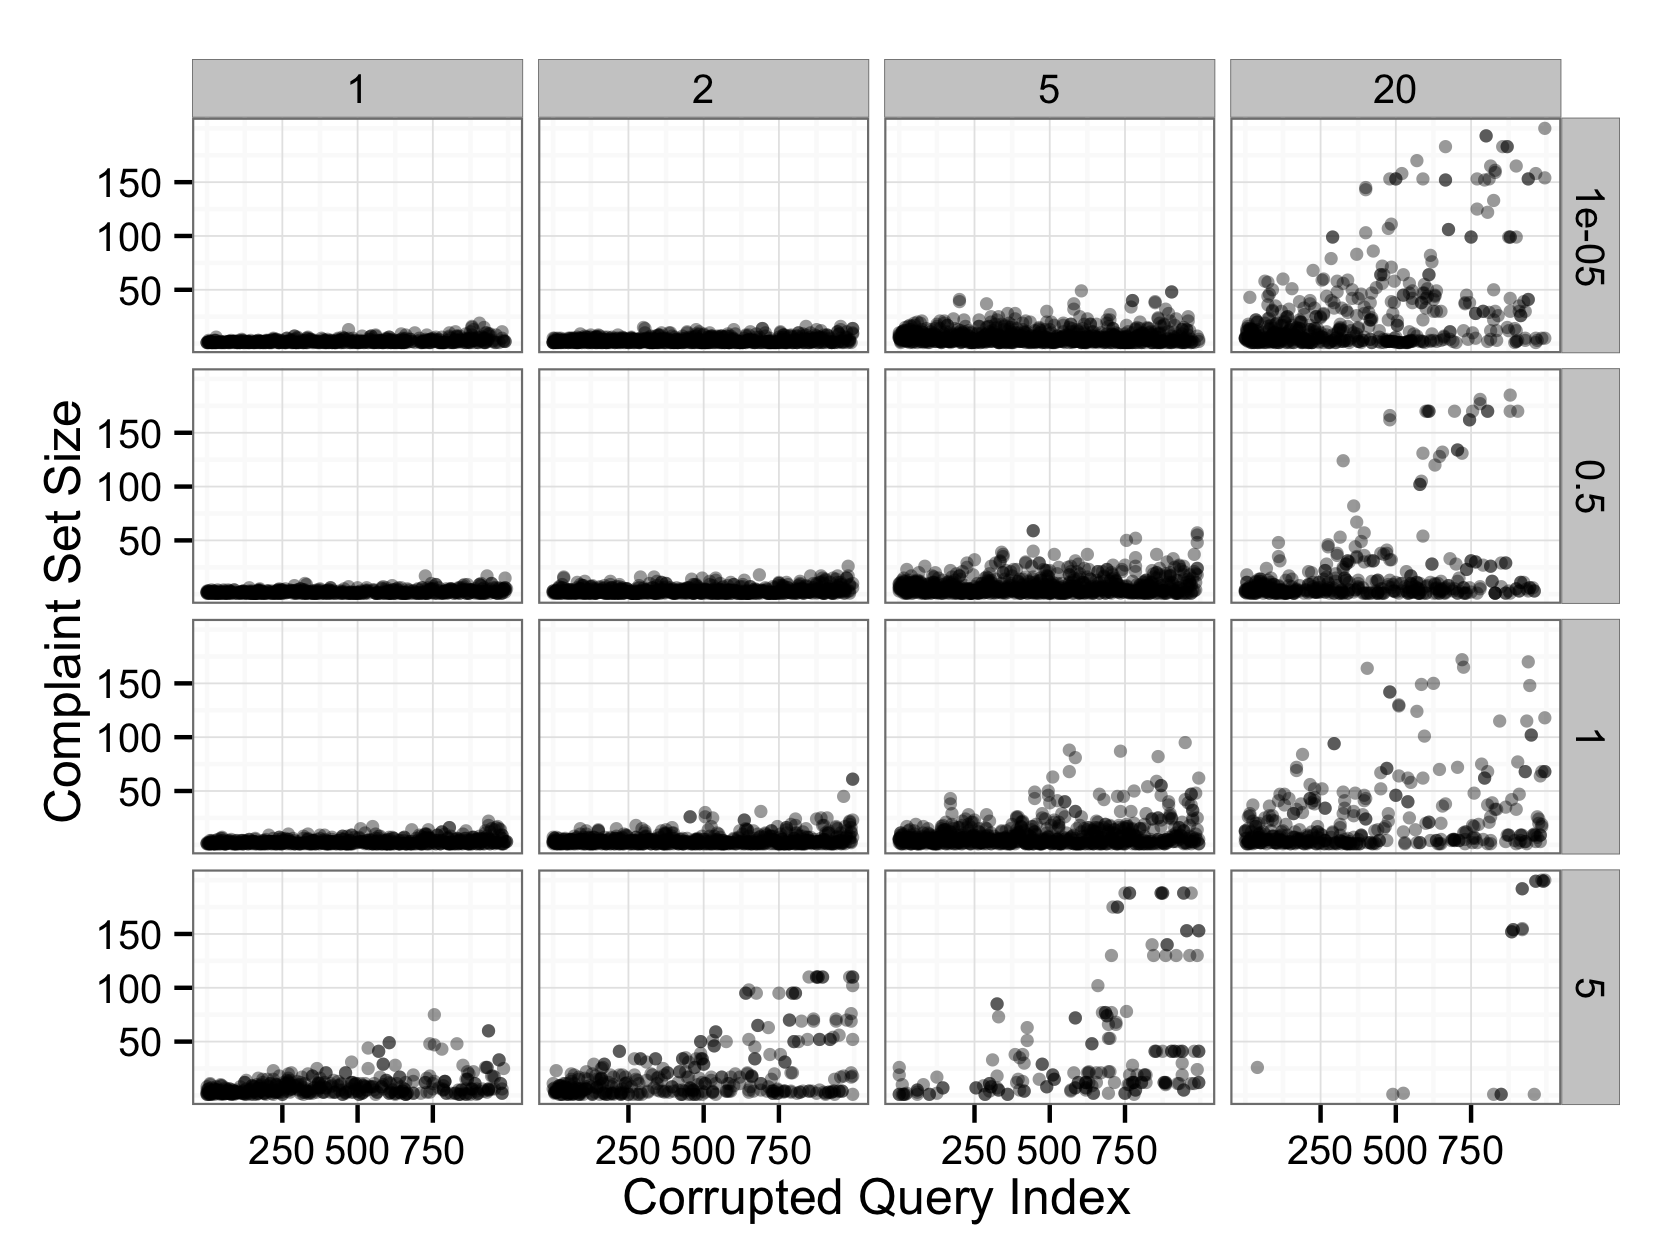
\includegraphics[width = 3.5in]{figures/qidxsimulation/qidx_v_ncomplaints_20attrs_const}
  \caption{Query index vs complaint set size for $set = const$.}
  \label{f:qidx_v_ncomplaints_const} 
  \end{figure}


Figure~\ref{f:qidx_v_ncomplaints_const} plots a representative set of parameters.  We plot one point
for each corrupted query index that results in a complaint set with at least one complaint. 
These results highlight several interesting trends.  When queries do not overlap ($r = 1$, leftmost column),
the size of the complaint sets are relatively small, and their frequency is constant across the possible query indices.
However as the possibility of overlap increases (e.g., $r$ increases), more recent queries are more likely to result in
very large complaint sets (at times the size of the database).   
This effect is a symptom of the fact that queries with large ranges will set groups of tuples to the same value,
and over time, skew the distribution of tuple values to a small number of possible values.
Thus, more recent corruptions that affect a large cluster of similar tuples will result in a large complaint set.
We find that increasing the skew parameter also exacerbates this effect.  
In addition, high skew increases the likelihood that queries will share the same \texttt{WHERE} and \texttt{SET} clause 
attributes as a corrupted query, thus overwriting the error introduced by the corrupted query.  
This is why the frequency of non-empty complaint sets decreases significantly as $s$ increases.


\begin{figure}[h]
\centering
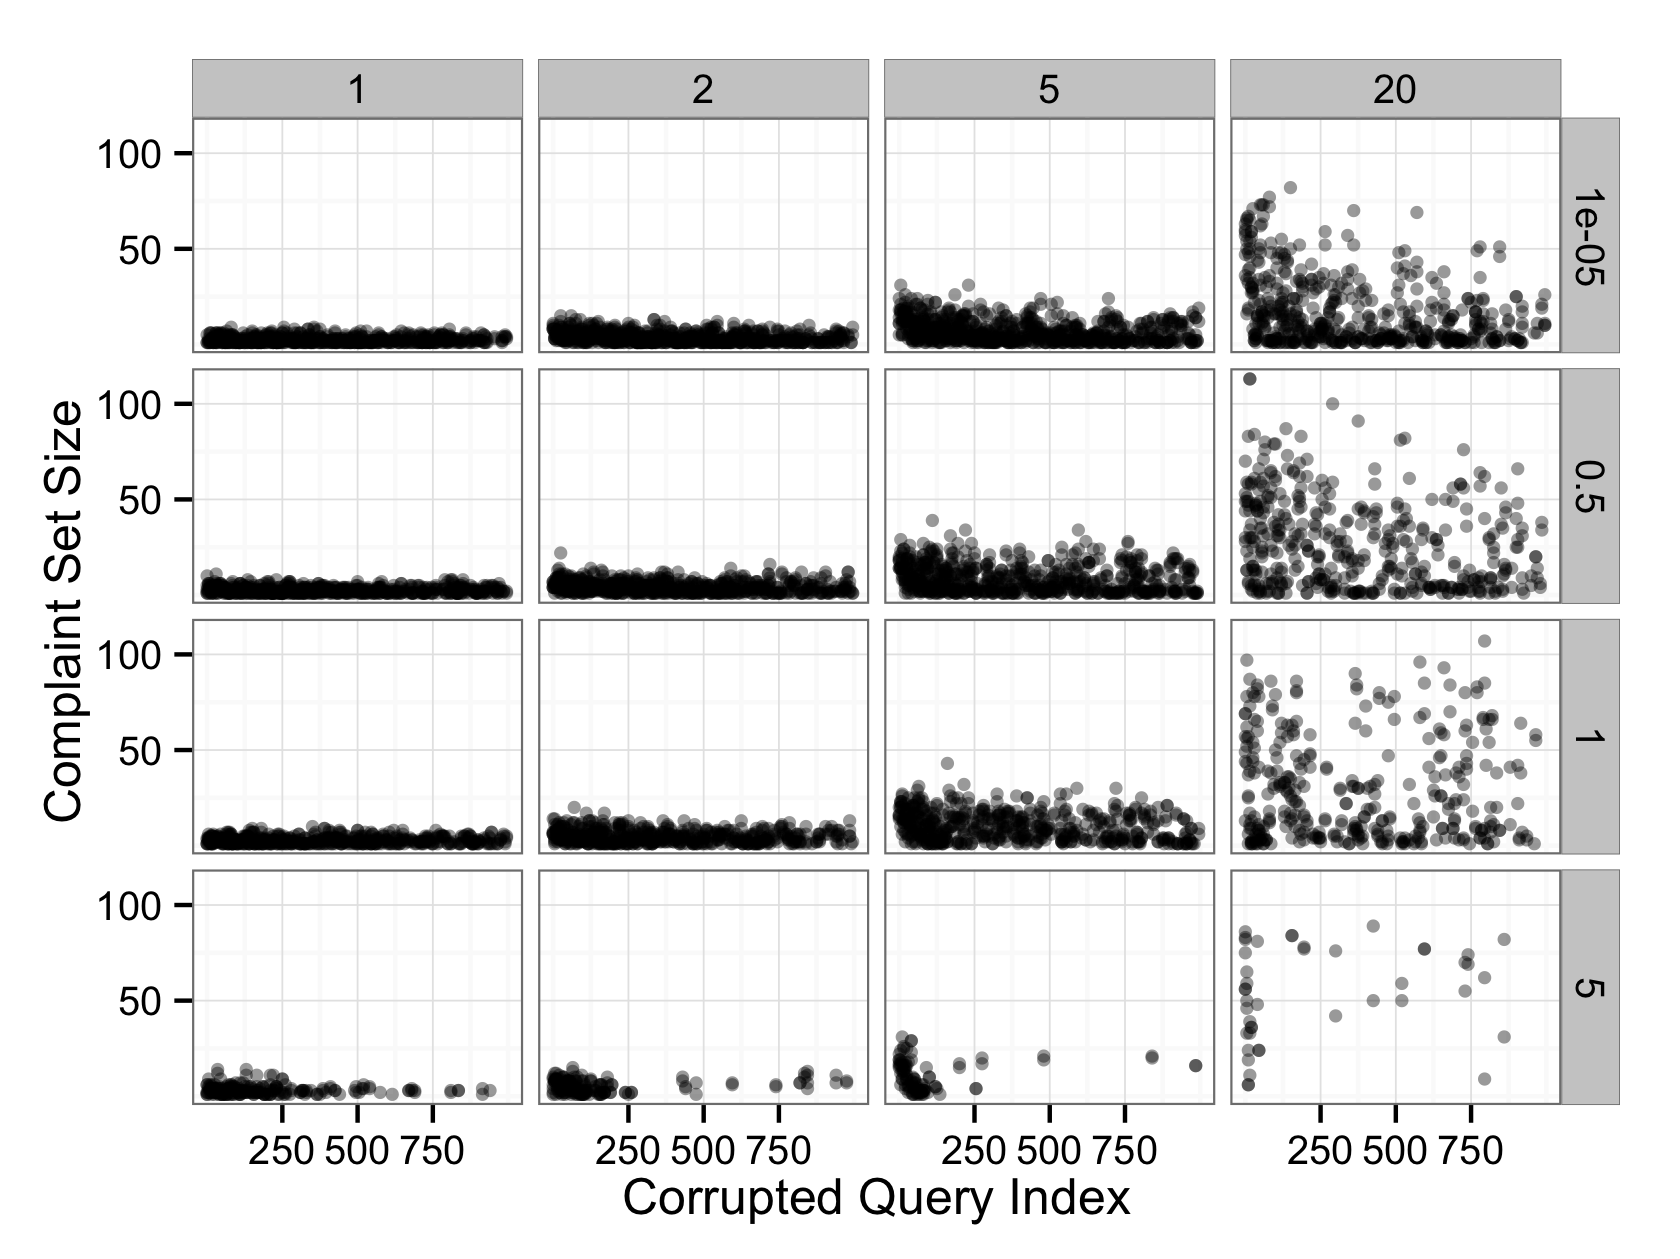
\includegraphics[width = 3.5in]{figures/qidxsimulation/qidx_v_ncomplaints_20attrs_rel}
\caption{Query index vs complaint set size for $set = rel$.}
\label{f:qidx_v_ncomplaints_rel} 
\end{figure}

In contrast to $set=const$ queries, Figure~\ref{f:qidx_v_ncomplaints_rel} executes the 
same experiment using $set=rel$ queries.  In this setting, we find that the trend is
reversed, and older corruptions tend to result in larger complaint sets.  This is because,
subsequent \texttt{UPDATE} queries increment or decrement the attribute value, rather than
overwriting it with a constant value.  The clustering of data values due to query overlap
then increases the number of other tuples affected.

% \begin{figure}[h]
% \centering
% 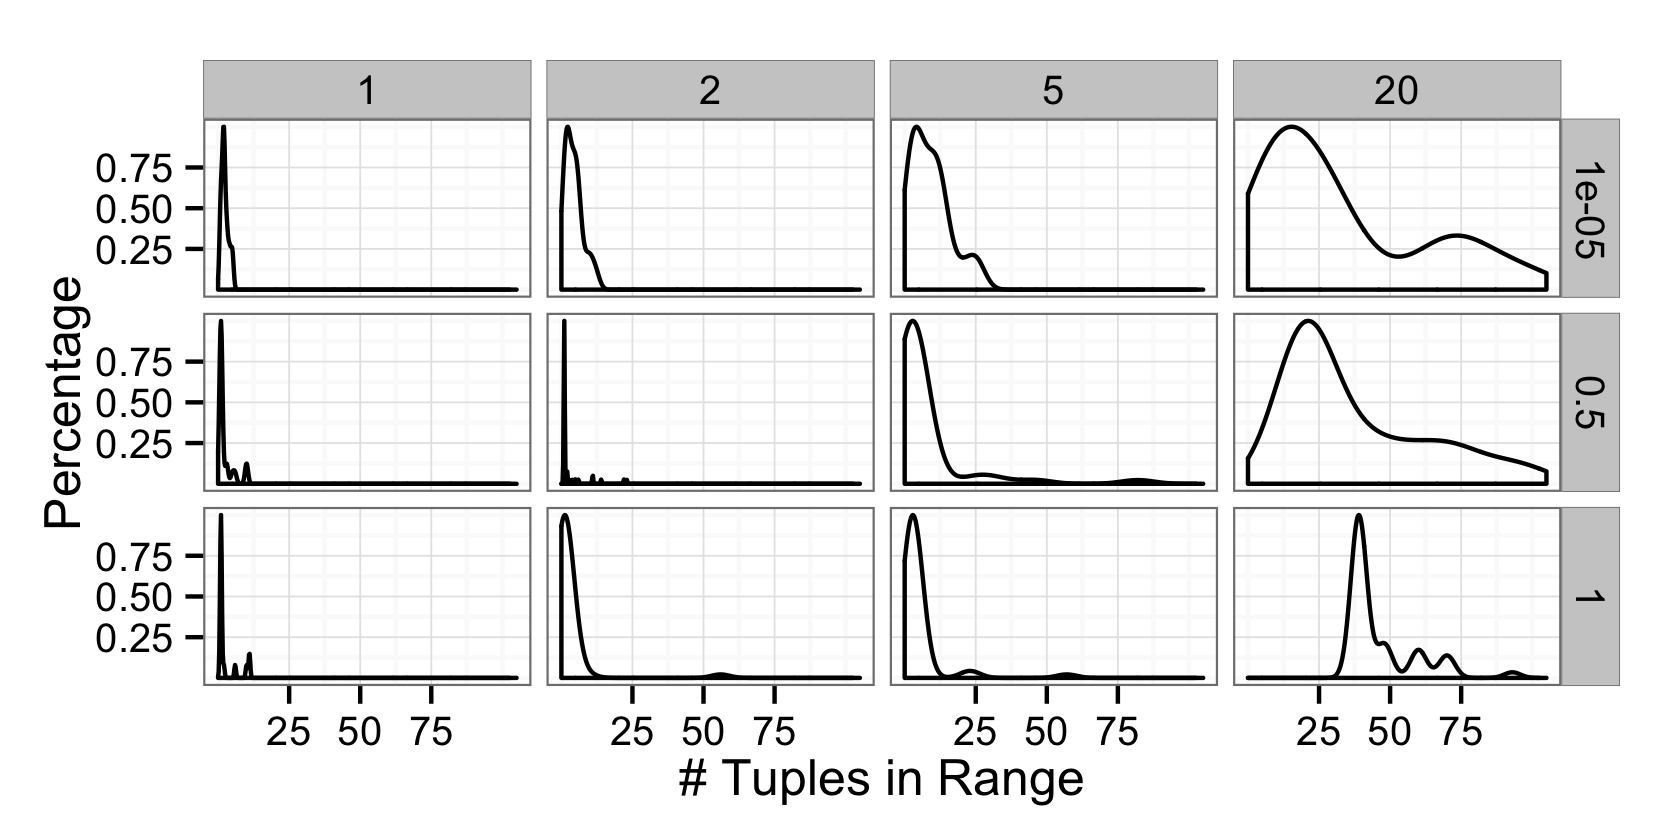
\includegraphics[width = 3.5in]{figures/qidxsimulation/numinrange}
% \caption{.}
% \label{f:numinrange} 
% \end{figure}



\subsection{Heuristics and Baseline Experiments}

\subsection{Skew}


\subsection{Scalabalitiy}




\subsection{Handling Noise}

In this set of experiments, we add false positive and false negative complaints to the input
complaint set and evaluate our noise handling algorithms (Section~\ref{sec:noise}).
To generate false positives ($FP$), we select a random set of tuples in the database, and for each one, 
pick a random attribute and set its XXX to a random value within $V_d$.
To generate false negatives ($FN$), we select a random subset of the true complaint set.


\begin{figure}[h]
\centering
  \begin{subfigure}[t]{.48\columnwidth}
  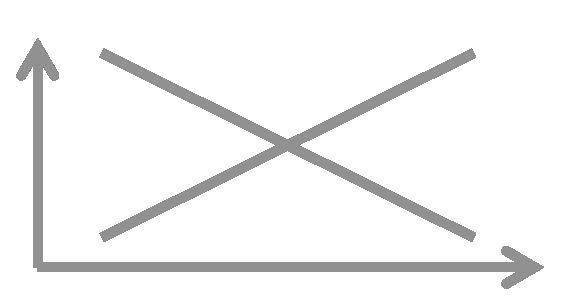
\includegraphics[width = .95\columnwidth]{figures/placeholder}
  \caption{.}
  \label{f:falsepositive} 
  \end{subfigure}
  \begin{subfigure}[t]{.48\columnwidth}
  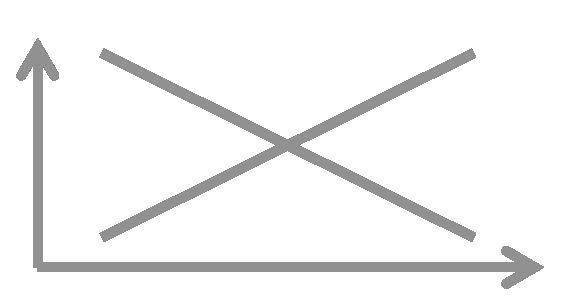
\includegraphics[width = .95\columnwidth]{figures/placeholder}
  \caption{.}
  \label{f:falsenegative} 
  \end{subfigure}
  \caption{cap}

\end{figure}



Figure~\ref{f:falsepositive} shows \sys performance and quality as we vary $FP \in \{\}$.

Figure~\ref{f:falsenegative} varies $FN \in \{\}$.


\subsection{Benchmark Experiments}














\iffalse
\subsubsection{Algorithms}

\sys fixes query logs in two distinct steps: first, we filter the query log using 
provenance information and roll back the queries to compute the $ideal$ states of the database.
Second, we apply the solver algorithms (Section~\ref{}) to speculatively fix the query.

We consider the roll-back algorithm in batches of $n_{rollback}$.

\begin{itemize}
\item Combined:  combine rollback and query fixing in a single CPLEX problem
\item $R_n-CPLEX$: 
\item DT
\item Box,Density
\end{itemize}



\subsubsection{Comparison}

\begin{itemize}
\item Query By Example algorithm
\item Quoc's ConQueR
\end{itemize}

Conditions, given a database ${\cal D}$ and query log $qlog$:

\begin{itemize}
\item {\bf $N_\mathcal{D}$: } Size of the database (number of tuples)
\item {\bf $N_{dim}$:} Dimensionality of the database.
\item {\bf $N_\mathcal{Q}$:} Vary number of queries in $qlog$.
\item {\bf $N_{pred}$:} The number of predicates in each UPDATE query's WHERE condition.
\item {\bf $N_{ins}$: } When corrupting the log, the number of values in INSERT to corrupt.
\item {\bf $N_{set}$: } When corrupting the log, the number of clauses in SET that are corrupted.
\item {\bf $N_{where}$: } When corrupting the log, the number of attributes in the WHERE clause that are corrupted.
\item {\bf $idx \in [0, 1]$: } The index of the query in the query log that was corrupted as a percentage of the query log.  
      For example $Idx = 0.0$ is the oldest query in the log, whereas $Idx = 1.0$ is the most recent query position.
\item {\bf $p_{I}$: } Percentage of INSERT queries in the query log (as compared to UPDATEs).
\item {\bf $p_{pk}$: } Percentage of UPDATE queries with primary key filter clauses as compared to range clauses over non-primary key attributes.
\item {\bf $p_{FP}$: } Percentage of false positives in the complaint set.
\item {\bf $p_{FN}$: } Percentage of false negatives in the complaint set.
\end{itemize}



\subsection{Exact Experiments}

\begin{itemize}
\item $N_\mathcal{D} \in \{10, 100, 1000\}$
\item $N_q \in \{10, 20, 50, 100\}$
\item $N_{dim} = 4$
\item $N_{pred} \in \{1, 2, 3\}$
\item $N_{where} = \{1, 2\}$
\item $Idx = \{0, 0.5, 1\}$
\end{itemize}

\subsection{Rollback and \qfix Microexperiments}


The first set of experiments seeks to understand the effectiveness of the database rollback
algorithm.  We use a synthetic dataset (\ewu{describe}) and execute the rollback algorithm
while varying the query batch size.

\subsection{End-to-end experiments}

\subsubsection{Complete Complaint Set}

\subsubsection{Complaint Set with Noise}

\begin{itemize}
\item $N_\mathcal{D} \in \{10, 100, 1000\}$
\item $N_q \in \{10, 20, 50, 100\}$
\item $N_{dim} = 4$
\item $N_{pred} \in \{1, 2, 3\}$
\item $N_{attrs} = \{1, 2\}$
\item $Idx = \{0, 0.5, 1\}$
\end{itemize}

\subsection{TPC-C Experiment}


\deprecate{
  \subsection{Single-Query Log}

  In the first set of experiments, we evaluate the simplest case where there
  is a single update query.  In each experiment, we vary the DBSize,
  NClauses, as well as the number of clauses in the query that have
  been corrupted and report the metrics described above.  We first 
  compare the learning algorithms on a complete complaint set, then evaluate them
  using incomplete complaint sets with varying percentages of false positive and negative complaints.

  \subsubsection{Complete Complaints}

  {\it Vary DBSize

  Vary NClauses, corrupt 1 and 2 clauses
  }

  We found that CPLEX and BBOX identify the correct fix, however their
  running times are significantly higher than DTree.  This is because
  CPLEX is an exact solution, as compared to DTree, whose poor early
  splitting decisions can adversely affect the final tree structure.

  \subsubsection{Incomplete Complaints}


  {\it 
  Vary DBSize

  Vary NClauses, corrupt 1 and 2 clauses

  Each line is plots has different perc FP
  }

  We first increased the number of false positives in the complaint set (no false negatives).
  Figure~\ref{f:single_incomplete_fp} shows how the fix quality and running time vary as the
  percentage of false positives increases.   Compared variations of CPlex and Bounding box with varying
  density thresholds (?).

  Each line varies perc FN

  We then varied the number of false negatives while keeping the percentage of false positives fixed at 5\%.
  Figure~\ref{f:single_incomplete_fn} 


  \subsection{Increased Query Log Size}

  In the following set of experiments, we increase the number of
  queries in the log while varying ?.  The number of corrupted queries
  is still one.  In these experiments, we set the DBSize to 10000,
  the default NClauses to 4, and the number of corrupted clauses to
  2.   We first show results for varying the false positives and
  negatives in the complaint set and comparing the algorithms described
  in Section~\ref{s:incomplete-algs}.  We then evaluate the efficacy
  of of provenance-based query log filtering, which reduces the running
  time without affecting the result quality.

  To generate the false-positives, we randomly sample without replacement
  from the tuples in the database that are not in the true complaint
  set.

  \subsection{False Positive}

  Vary false positives (1 graph)


  \subsection{False Negative}

  Vary false negatives (1 graph)

  \subsubsection{Filtering Queries}

  We also compared the provenance-based filtering techniques in the above experiments
  to measure their effectiveness at reducing the running time.  We varied the complexity of the update 
  WHERE clauses to control the amount that queries in the log overlap in their updates.  The query log contained 50 update WHERE queries.
  The quality of the suggested fixes were the same,  As the clauses became less complex, the likelihood 
  of overlap increased, and increased the amount of queries that affected the complaint sets.


  \begin{figure}[h]
  \centering
  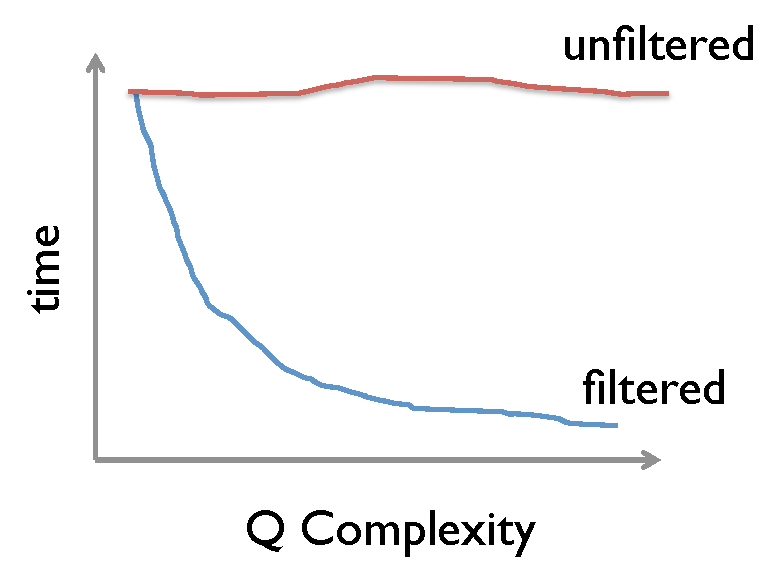
\includegraphics[width = 2in]{figures/complete_qfilter_complexity}
  \caption{Varying query complexity.}
  \label{f:complete_qfilter_complexity} 
  \end{figure}



  \subsection{Multi-Query}

  Using a previous experimental configuration, we varied the number of queries that are corrupted.  Figures~\ref{}
  show the quality and running times of the results for a query log of size 1000 and dbsize of 100k.  
  As we can see, the cost increases quadratically with each corrupted query and the accuracy of the proposed fixes increases marginally.  
  This is because XXX.

  We focus on two scenarios.  {\bf Try multiple corruptions that don't overlap (provenance-wise) with each other}.  This is the condition of multiple silo'd that
  corrupt their own logs.  Then {\bf Try multiple corrupted queries where one query modifies the updated state of the other}.  This shows that
  it is really hard and hopefully we get close?



  To better understand the algorithm, we plot the quality metrics after each fixed query and measure how quickly \sys converges to the final result. 
  This suggests that an incremental approach where the user can set a threshold to stop the algorithm may be effective.



  \subsection{Real Transactional Workload}

  We used the web application workload, and evaluated our alogirthms with artifically injected corruptions.
  We compared two types of corruptinos.  In figure~\ref{f:real_existing}, we randomly picked a single existing 
  query and corrupted its value.  If the query was an INSERT, we randomly pick a value and perturbed it.
  If the transaction was an UPDAET, we randomly varied the SET or WHERE clauses.   We re-ran this
  100 times and plot the average and standard deviation of the results.

}
\fi
